\documentclass[a4paper,12pt]{extarticle}
\usepackage[utf8x]{inputenc}
\usepackage[T1,T2A]{fontenc}
\usepackage[russian]{babel}
\usepackage{hyperref}
\usepackage{indentfirst}
\usepackage{listings}
\usepackage{color}
\usepackage{here}
\usepackage{array}
\usepackage{multirow}
\usepackage{graphicx}
\usepackage{amsmath}
\usepackage{amssymb}
\usepackage{makeidx}    

\usepackage{caption}
\renewcommand{\lstlistingname}{Программа} % заголовок листингов кода

\bibliographystyle{ugost2008ls}

\usepackage{listings}
\lstset{ %
extendedchars=\true,
keepspaces=true,
language=C,						% choose the language of the code
basicstyle=\footnotesize,		% the size of the fonts that are used for the code
numbers=left,					% where to put the line-numbers
numberstyle=\footnotesize,		% the size of the fonts that are used for the line-numbers
stepnumber=1,					% the step between two line-numbers. If it is 1 each line will be numbered
numbersep=5pt,					% how far the line-numbers are from the code
backgroundcolor=\color{white},	% choose the background color. You must add \usepackage{color}
showspaces=false				% show spaces adding particular underscores
showstringspaces=false,			% underline spaces within strings
showtabs=false,					% show tabs within strings adding particular underscores
frame=single,           		% adds a frame around the code
tabsize=2,						% sets default tabsize to 2 spaces
captionpos=t,					% sets the caption-position to top
breaklines=true,				% sets automatic line breaking
breakatwhitespace=false,		% sets if automatic breaks should only happen at whitespace
escapeinside={\%*}{*)},			% if you want to add a comment within your code
postbreak=\raisebox{0ex}[0ex][0ex]{\ensuremath{\color{red}\hookrightarrow\space}},
texcl=true,
inputpath=source,                     % директория с листингами
}

\usepackage[left=2cm,right=2cm,
top=2cm,bottom=2cm,bindingoffset=0cm]{geometry}

%% Нумерация картинок по секциям
\usepackage{chngcntr}
\counterwithin{figure}{section}
\counterwithin{table}{section}

%%Точки нумерации заголовков
\usepackage{titlesec}
\titlelabel{\thetitle.\quad}
\usepackage[dotinlabels]{titletoc}

%% Оформления подписи рисунка
\addto\captionsrussian{\renewcommand{\figurename}{Рисунок}}
\captionsetup[figure]{labelsep = period}

%% Подпись таблицы
\DeclareCaptionFormat{hfillstart}{\hfill#1#2#3\par}
\captionsetup[table]{format=hfillstart,labelsep=newline,justification=centering,skip=-10pt,textfont=bf}

%% Путь к каталогу с рисунками
\graphicspath{{pictures/}}


\begin{document}	% начало документа

% Титульная страница
\begin{titlepage}	% начало титульной страницы

	\begin{center}		% выравнивание по центру

		\large Санкт-Петербургский Политехнический Университет Петра Великого\\
		\large Институт компьютерных наук и технологий \\
		\large Кафедра компьютерных систем и программных технологий\\[6cm]
		% название института, затем отступ 6см
		
		\huge Телекоммуникационные технологии\\[0.5cm] % название работы, затем отступ 				%0,5см
		\large Отчет по лабораторной работе №3\\[0.1cm]
		\large Линейная фильтрация
		\\[5cm]

	\end{center}


	\begin{flushright} % выравнивание по правому краю
		\begin{minipage}{0.25\textwidth} % врезка в половину ширины текста
			\begin{flushleft} % выровнять её содержимое по левому краю

				\large\textbf{Работу выполнил:}\\
				\large Балсутьев В.А.\\
				\large {Группа:} 33501/4\\
				
				\large \textbf{Преподаватель:}\\
				\large Богач Н.В.

			\end{flushleft}
		\end{minipage}
	\end{flushright}
	
	\vfill % заполнить всё доступное ниже пространство

	\begin{center}
	\large Санкт-Петербург\\
	\large \the\year % вывести дату
	\end{center} % закончить выравнивание по центру

\thispagestyle{empty} % не нумеровать страницу
\end{titlepage} % конец титульной страницы

\vfill % заполнить всё доступное ниже пространство
	

% Содержание
% Содержание
\renewcommand\contentsname{\centerline{Содержание}}
\tableofcontents
\newpage




\section{Цель работы}
Получить представление о спектрах телекоммуникационных
сигналов.

\section{Постановка задачи}

\begin{itemize}

\item Для сигналов, построенных в лабораторной работе No1, выполните расчет преобразования Фурье, получите спектры.
\item  С помощью функции корреляции найдите позицию синхропосылки [101] в сигнале [0001010111000010]. Получите пакет
данных, если известно, что его длина составляет 8 бит без
учета синхропосылки. Вычислите корреляцию прямым методом, воспользуйтесь алгоритмом быстрой корреляции, сравните время работы обоих алгоритмов.
\item Теоретические положения к лабораторной работе: Справочные материалы: А.Б.Сергиенко Цифровая обработка сигналов. Глава 1,  сс.25–55, Глава 5, сс. 284–285.

\end{itemize}



\section{Теоретическая информация}
\subsection{Ряд Фурье}
Разложению в ряд Фурье могут подвергаться периодические сигналы. При этом они представляютсяв виде суммы гармонических функций либо комплексных экспонент с частотами, образующими арифметическую прогрессию. Для того чтобы такое разложение существовало, рагмент сигнала длительностью в один период должен удовлетворять условиям Дирихле:

\begin{itemize}
\item не должно быть разрывов второго рода(с уходящими в бесконечность ветвями функции)
\item число разрывов первого рода (скачков) должно быть конечным
\item число экстремумов должно быть конечным(в качестве примера функуции, которая
на конечном интервале имеет бесконечное число экстремумов, можно привести $\sin(1/x)$ в окрестности нуля)
\end{itemize}
\noindent В зависимости от конкретной формы базисных функций различают несколько форм записи ряда Фурье. \\
Следует отметить, что ряд Фурье может быть применен для разложения и не периодические сигналы. При этом оговаривается временной интервал, для которого строится ряд Фурье, а 
в остальные моменты времени сигнал считается равным нулю. \\
\noindent Как уже было сказано выше существуют несколько форм представления ряда Фурье:

\begin{itemize}
\item Синусно-косинусная форма \\
$$ s(t) = \frac{a_0}{2} +  \sum\limits_{k=1}^{\infty}(a_k \cos(k \omega_1 t) + b_k \sin(k \omega_1 t)) $$
В данной формуле $\omega_1 = 2 \pi / T$ - круговая частота, соответствующая периоду повторения сигнала, равному $T$. Входящие в в формулу кратные ей частоты $ k \omega_1 $
называются гармониками($ k $ - ая гармоника $ k \omega_1 $).
  
\item Вещественнная форма \\
Некоторое неудобство предыдущей формы заключается в том, что для каждого значения индекса суммирования $k$ в формуле фигурируют два слагаемых - синус и косинус. С помощью 
тригонометрических формул и не хитрых преобразований можно синусно-косинусную форму привести к более короткой записи:
$$s(t) = \frac{a_0}{2} +  \sum\limits_{k=1}^{\infty}(A_k \cos(k \omega_1 t + \phi_k ) $$
\item Комплексная форма \\
Данная форма представления ряда Фурье является самой общей, поскольку охватывает надмножество вещественных чисел - комплексные.Данная форма получается подставлением
косинуса в виде полусуммы комплексных экспонент (следствие из \href{https://ru.wikipedia.org/wiki/%D0%A4%D0%BE%D1%80%D0%BC%D1%83%D0%BB%D0%B0_%D0%AD%D0%B9%D0%BB%D0%B5%D1%80%D0%B0}{формулы Эйлера}):

$$ \cos x = \frac{1}{2}(e^{jx} + e^{-jx}) $$ 

Применив данное преобразование к вещественной форме ряда Фурье, получим суммы комплексных экспонент с положительными и отрицательными показателями:

$$ s(t) = \frac{a_0}{2} +  \sum\limits_{k=1}^{\infty} \frac{A_k}{2} 
(\exp(jk \omega_1 t + j \phi_k) + \exp(-jk \omega_1 t - j \phi_k)) $$

Теперь будем трактовать экспоненты со знаком минус в показателе как члены ряда с отрицательными номерами. В рамках этого же общего подхода постоянное слагаемое $ a_0 / 2$ станет членом ряда с нулевым номером. В результате получится комплексная форма записи ряда Фурье:

$$  \sum\limits_{k=1}^{\infty}C_k e^{-jk \omega_1t} $$ 

Из чего следует, что коэффициенты $ С_k $ ряда Фурье в комплексной форме можно рассчитать по формуле:
$$ C_k = \frac{1}{T}  \int_{-T/2}^{T/2} s(t) \exp(-jk \omega_1) dt $$
Совокупнсть амплитуд гармоник ряда Фурье часто называют амплитудным спектром, а совокупность их фаз - фазовым спектром.  

\subsection{ Преобразование Фурье}

Как уже было сказано выше, основной формой представления ряда Фурье является комплексная
и при помощи достаточно сложных математических выводов, нетревиальных переходов и рассуждений получаем из формулы ряда Фурье формулу прямого преобразования Фурье, с помощью которой будем находить спектры, а значит и осуществлять спектральный анализ:

$$ S(\omega ) = \int_{-\infty}^{\infty} s(t)e^{-jk \omega t} dt $$

\noindent В данном случае $ S(\omega ) $ не что иное, как комплексный коэффициент ряда Фурье, именно после вычисления данных коэффициентов можно строить спектры и именно данные коэффициенты возвращает функция fft как MATLAB, так и в python. \\  
Также существует формула обратного преобразования Фурье, которая нам пригодится для вычисления быстрой корреляции:

$$ s(t) = \frac{1}{2 \pi} \int_{-\infty}^{\infty} S(\omega)e^{-jk \omega t} d \omega $$

    
\end{itemize}
 


\section{Ход работы}

\subsection{Гармонический сигнал}
Для начала построим гармонический сигнал $s_1(t) = \cos(2\pi f_0t +\phi)$
и с помощью пэкиджа fftpack из scipy построим спектр:
\lstinputlisting[
	label=code:source01,
	caption={source01.py},% для печати символ '_' требует выходной символ '\'
]{source01.py}
\parindent=1cm % командна \lstinputlisting сбивает параментры отступа

Получаем в результате интерпретации нашей программы графики исходного сигнала и
его спектр:

\begin{figure}[H]
	\begin{center}
		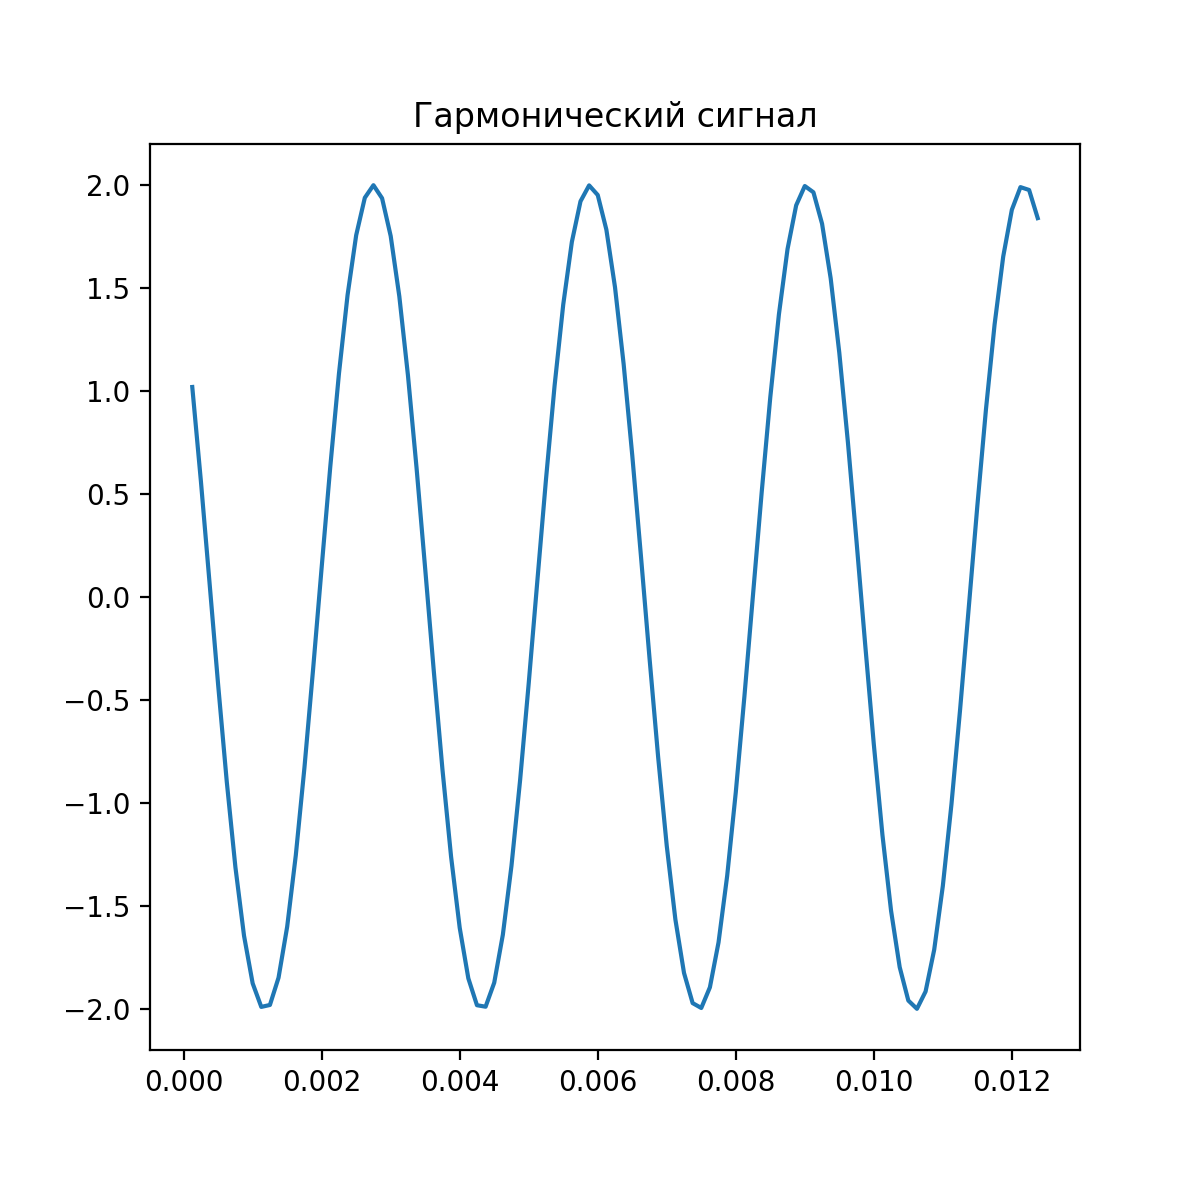
\includegraphics[scale=0.7]{001_1harmonic.png}
		\caption{Гармонический сигнал} 
		\label{pic:pic01} % название для ссылок внутри кода
	\end{center}
\end{figure} 

\begin{figure}[H]
	\begin{center}
		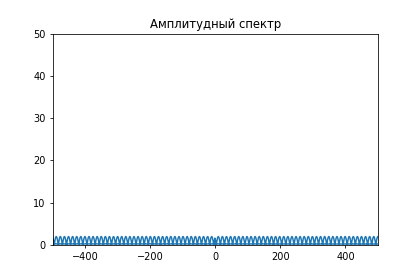
\includegraphics[scale=0.7]{001_2harmspectr.png}
		\caption{Амплитудный спектр} 
		\label{pic:pic02} % название для ссылок внутри кода
	\end{center}
\end{figure} 

\subsection{Прямоугольный импульс}

Из-за отсутствия функции одиночного импульса в scipy.signal реализуем
собственную rectimpls(t, width), где t - время в секундах, width - 
ширина импульса также в секундах. И повторим 
процедуру построения спектра c помощью fftpack: 

\lstinputlisting[
	label=code:source02,
	caption={source02.py},% для печати символ '_' требует выходной символ '\'
]{source02.py}
\parindent=1cm % командна \lstinputlisting сбивает параментры отступа

Получаем в качестве спектра ожидаемый $s(f) = sinc(f)$ 

\begin{figure}[H]
	\begin{center}
		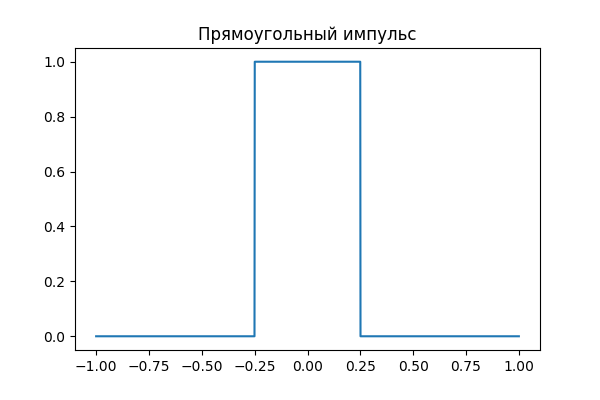
\includegraphics[scale=0.7]{002_1rectImpl.png}
		\caption{Прямоугольный импульс} 
		\label{pic:pic03} % название для ссылок внутри кода
	\end{center}
\end{figure} 

\begin{figure}[H]
	\begin{center}
		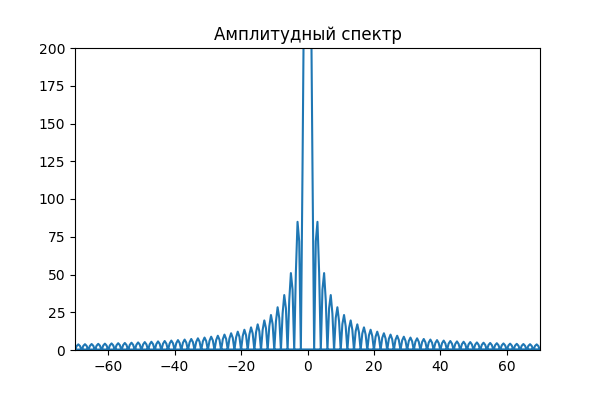
\includegraphics[scale=0.7]{002_2rectImplSpectr.png}
		\caption{Амплитудный спектр} 
		\label{pic:pic04} % название для ссылок внутри кода
	\end{center}
\end{figure} 

\subsection{Периодический прямоугольный сигнал}
Далее проведем тот же эксперимент для периодического прямоугольного сигнала:

\lstinputlisting[
	label=code:source03,
	caption={source03.py},% для печати символ '_' требует выходной символ '\'
]{source03.py}
\parindent=1cm % командна \lstinputlisting сбивает параментры отступа

%Получаем в качестве спектра ожидаемый %$s(f) = sinc(f)$ 
Получаем в соотвествии с теорией:
\begin{figure}[H]
	\begin{center}
		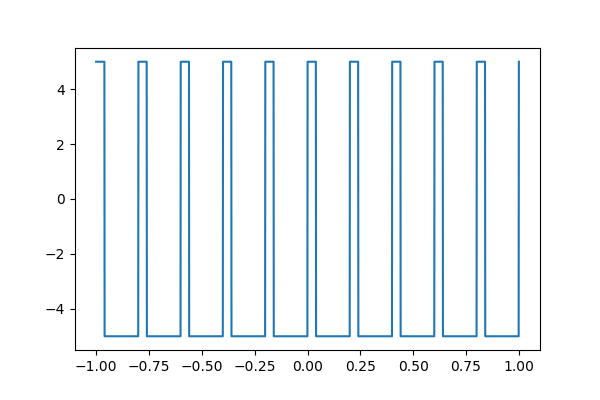
\includegraphics[scale=0.7]{003_1rectImplses.png}
		\caption{Прямоугольный сигнал} 
		\label{pic:pic05} % название для ссылок внутри кода
	\end{center}
\end{figure} 

\begin{figure}[H]
	\begin{center}
		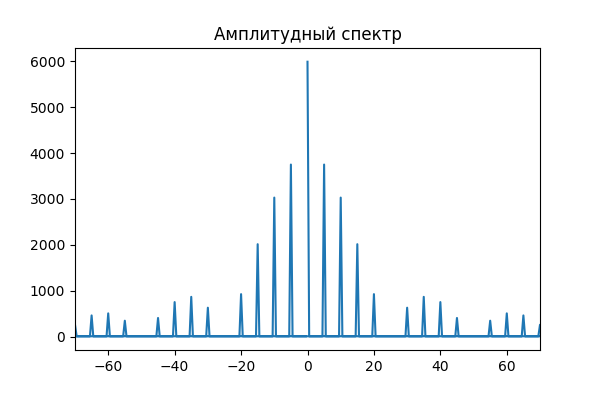
\includegraphics[scale=0.7]{003_2rectImplSpectr.png}
		\caption{Амплитудный спектр} 
		\label{pic:pic06} % название для ссылок внутри кода
	\end{center}
\end{figure} 

\subsection{Пилообразный сигнал}
Воспользовавшись стандартной функцией  sawtooth из scipy.signal строим пилообразный сигнал и далее его  спектр:
\lstinputlisting[
	label=code:source04,
	caption={source04.py},% для печати символ '_' требует выходной символ '\'
]{source04.py}
\parindent=1cm % командна \lstinputlisting сбивает параментры отступа

%Получаем в качестве спектра ожидаемый %$s(f) = sinc(f)$ 
Получаем в соотвествии с теорией:
\begin{figure}[H]
	\begin{center}
		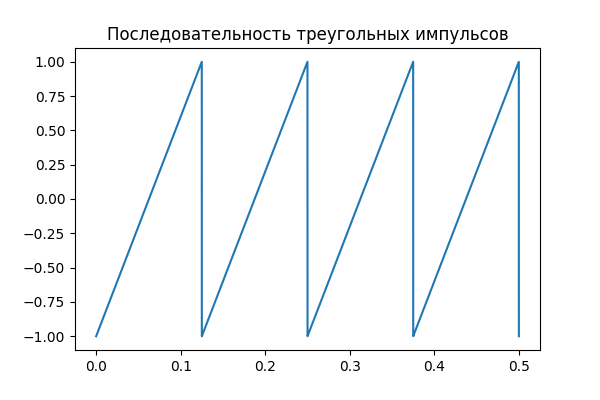
\includegraphics[scale=0.7]{004_1sawtooth.png}
		\caption{Пилообразный сигнал} 
		\label{pic:pic07} % название для ссылок внутри кода
	\end{center}
\end{figure} 

\begin{figure}[H]
	\begin{center}
		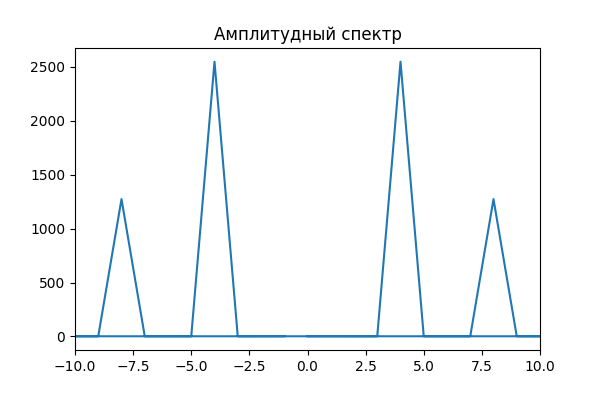
\includegraphics[scale=0.7]{004_2sawToothSpectr.png}
		\caption{Амплитудный спектр} 
		\label{pic:pic08} % название для ссылок внутри кода
	\end{center}
\end{figure} 


\subsection{Функция Дирихле}
С помощью diric из scipy.special сигнал соотвествии с формулой Дирихле:
	%\begin{equation}\label{eq4}  
$$	\frac{\sin(nx/2)}{nsin(nx/2)}, n \in \mathbb Z $$ 			
	%\end{equation}
%$$ s(t) = \frac{1}{2 \pi} \int_{-\infty}^{\infty} S(\omega)e^{-jk \omega t} d \omega $$

и далее его  спектр для степеней n = 7 и 8 соотвественно:

\lstinputlisting[
	label=code:source05,
	caption={source05.py},% для печати символ '_' требует выходной символ '\'
]{source05.py}
\parindent=1cm % командна \lstinputlisting сбивает параментры отступа

%Получаем в качестве спектра ожидаемый %$s(f) = sinc(f)$ 
Получаем в соотвествии с теорией:
\begin{figure}[H]
	\begin{center}
		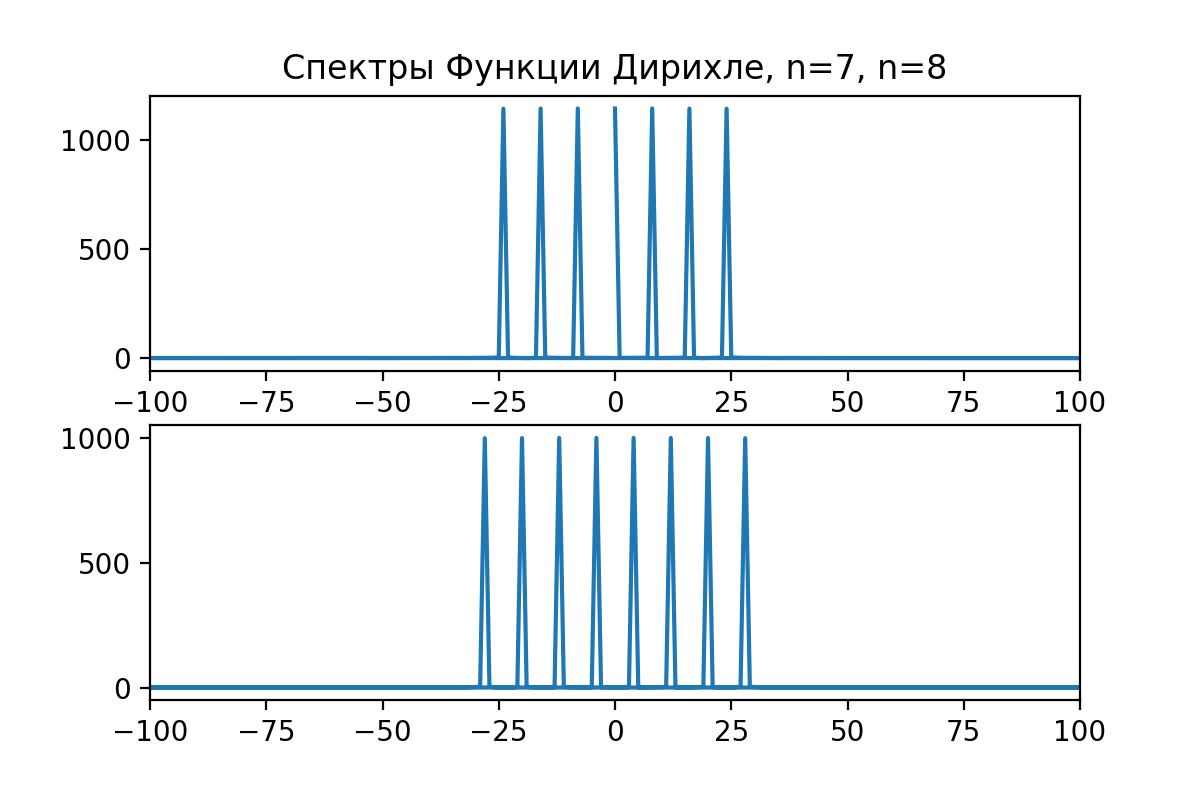
\includegraphics[scale=0.7]{005_1dirichle.png}
		\caption{Функции Дирихле} 
		\label{pic:pic09} % название для ссылок внутри кода
	\end{center}
\end{figure} 

\begin{figure}[H]
	\begin{center}
		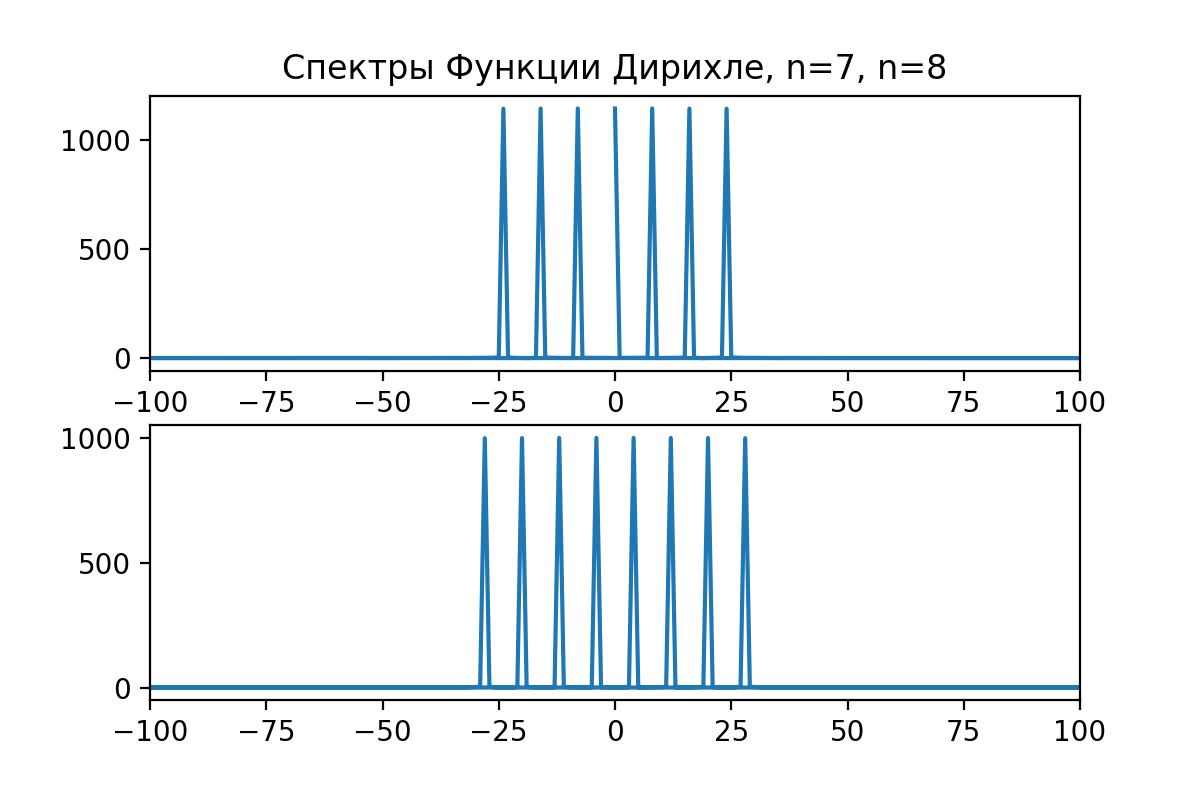
\includegraphics[scale=0.7]{005_2dirichleSpectr.png}
		\caption{Амплитудный спектр} 
		\label{pic:pic010} % название для ссылок внутри кода
	\end{center}
\end{figure} 

\subsection{Корреляция}
Найдя функцию для вычисления корреляции в scipy.signal, найдем корреляцию.
Далее в соответсвии с \href{http://www.williamspublishing.com/PDF/5-8459-0710-1/part.pdf}{пособием}
из которого мы взяли формулу вычисления быстрой корреляции(стр 303 параграф 5.2.3):

$$ r(j) = \frac{F_D^{-1}[X_1^*(k)X_2(k)]}{N},  $$

где r - корреляция, $F_D^{-1}$ - обратное   дискретное преобразования Фурье, $N$ - степень дискретизации, $X_1(k), X_2(k)$ - ДПФ - образы для периодических последовательностей $x_1(l), x_2(r)$, корреляцию которых считаем.
  
\lstinputlisting[
	label=code:source06,
	caption={source06.py},% для печати символ '_' требует выходной символ '\'
]{source06.py}
\parindent=1cm % командна \lstinputlisting сбивает параментры отступа

Выполняем сценарий и получаем:

\begin{figure}[H]
	\begin{center}
		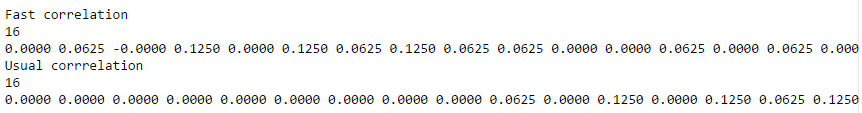
\includegraphics[scale=0.7]{corr.png}
		\caption{Корреляция} 
		\label{pic:pic011} % название для ссылок внутри кода
	\end{center}
\end{figure} 


\section{Вывод}
Таким образом мы рассмотрели преобразование Фурье и научились находить его для различных сигналов 
с помощью библиотеки python-scipy.signal. 
Следует отметить, что преобразование Фурье в обработке сигналов обычно рассматривается как декомпозиция 
сигнала на частоты и амплитуды, то есть обратимый переход от временного пространства в частотное пространство.

 

\end{document}
